%%%%%%%%%%%%%%%%%%%%%%%%%%%%%%%%%%%%%%%%%
% Journal Article
% LaTeX Template
% Version 1.4 (15/5/16)
%
% This template has been downloaded from:
% http://www.LaTeXTemplates.com
%
% Original author:
% Frits Wenneker (http://www.howtotex.com) with extensive modifications by
% Vel (vel@LaTeXTemplates.com)
%
% License:
% CC BY-NC-SA 3.0 (http://creativecommons.org/licenses/by-nc-sa/3.0/)
%
%%%%%%%%%%%%%%%%%%%%%%%%%%%%%%%%%%%%%%%%%

%----------------------------------------------------------------------------------------
%	PACKAGES AND OTHER DOCUMENT CONFIGURATIONS
%----------------------------------------------------------------------------------------

\documentclass[twoside,twocolumn]{article}

\usepackage{blindtext} % Package to generate dummy text throughout this template

\usepackage[sc]{mathpazo} % Use the Palatino font
\usepackage[T1]{fontenc} % Use 8-bit encoding that has 256 glyphs
\linespread{1.05} % Line spacing - Palatino needs more space between lines
\usepackage{microtype} % Slightly tweak font spacing for aesthetics

\usepackage[english]{babel} % Language hyphenation and typographical rules

\usepackage[hmarginratio=1:1,top=32mm,columnsep=20pt]{geometry} % Document margins
\usepackage[hang, small,labelfont=bf,up,textfont=it,up]{caption} % Custom captions under/above floats in tables or figures
\usepackage{booktabs} % Horizontal rules in tables

\usepackage{lettrine} % The lettrine is the first enlarged letter at the beginning of the text

\usepackage{enumitem} % Customized lists
\setlist[itemize]{noitemsep} % Make itemize lists more compact

\usepackage{abstract} % Allows abstract customization
\renewcommand{\abstractnamefont}{\normalfont\bfseries} % Set the "Abstract" text to bold
\renewcommand{\abstracttextfont}{\normalfont\small\itshape} % Set the abstract itself to small italic text

\usepackage{titlesec} % Allows customization of titles
\renewcommand\thesection{\Roman{section}} % Roman numerals for the sections
\renewcommand\thesubsection{\roman{subsection}} % roman numerals for subsections
\titleformat{\section}[block]{\large\scshape\centering}{\thesection.}{1em}{} % Change the look of the section titles
\titleformat{\subsection}[block]{\large}{\thesubsection.}{1em}{} % Change the look of the section titles

\usepackage{fancyhdr} % Headers and footers
% \pagestyle{fancy} % All pages have headers and footers
\fancyhead{} % Blank out the default header
\fancyfoot{} % Blank out the default footer
%\fancyhead[C]{Running title $\bullet$ May 2016 $\bullet$ Vol. XXI, No. 1} % Custom header text
\fancyfoot[RO,LE]{\thepage} % Custom footer text

\usepackage{titling} % Customizing the title section

\usepackage{hyperref} % For hyperlinks in the PDF


\usepackage{graphicx} % For inserting images
\graphicspath{ {images/} } % Folder where images are stored

%----------------------------------------------------------------------------------------
%	TITLE SECTION
%----------------------------------------------------------------------------------------

\setlength{\droptitle}{-4\baselineskip} % Move the title up

\pretitle{\begin{center}\Huge\bfseries} % Article title formatting
\posttitle{\end{center}} % Article title closing formatting
\title{SYDE 351 Project Report} % Article title
\author{%
\textsc{Krishn Ramesh, 20521942} \\[1ex]
\and
\textsc{Kevin Michael, 20507239} \\[1ex]
\and
\textsc{Peter Gokhshteyn, 20508507} \\[1ex]
}
\date{July 26, 2016} % Leave empty to omit a date

\renewcommand{\maketitlehookd}{%
\begin{abstract}
% TODO @kevin: finish the abstract
\noindent \blindtext % Dummy abstract text - replace \blindtext with your abstract text
\end{abstract}
}

%----------------------------------------------------------------------------------------

\begin{document}

% Print the title
\maketitle

%----------------------------------------------------------------------------------------
%	ARTICLE CONTENTS
%----------------------------------------------------------------------------------------

\section{Introduction}

\lettrine[nindent=0em,lines=3]{I} nteresting dynamic behaviours can be found everywhere, but as simple as they may seem at first glance, their internal workings can be quite tricky to study. Systems Design Engineers, in particular, need to be proficient at modeling complex systems. To practice this skill, the SYDE 351 course has a modeling \& simulation project. A simple prototype was chosen to be built, taking inspiration from the chain mechanism of bicycles. The prototype, seen in Figure 1, is composed of two wheels of varying sizes. Physically, the user rotates the top wheel which in turn rotates the bottom wheel. The bottom wheel slips suddenly every rotation due to the elastics that connect both wheels.

\begin{figure}[!ht]
    \caption{Photograph of the prototype}
    \centering
        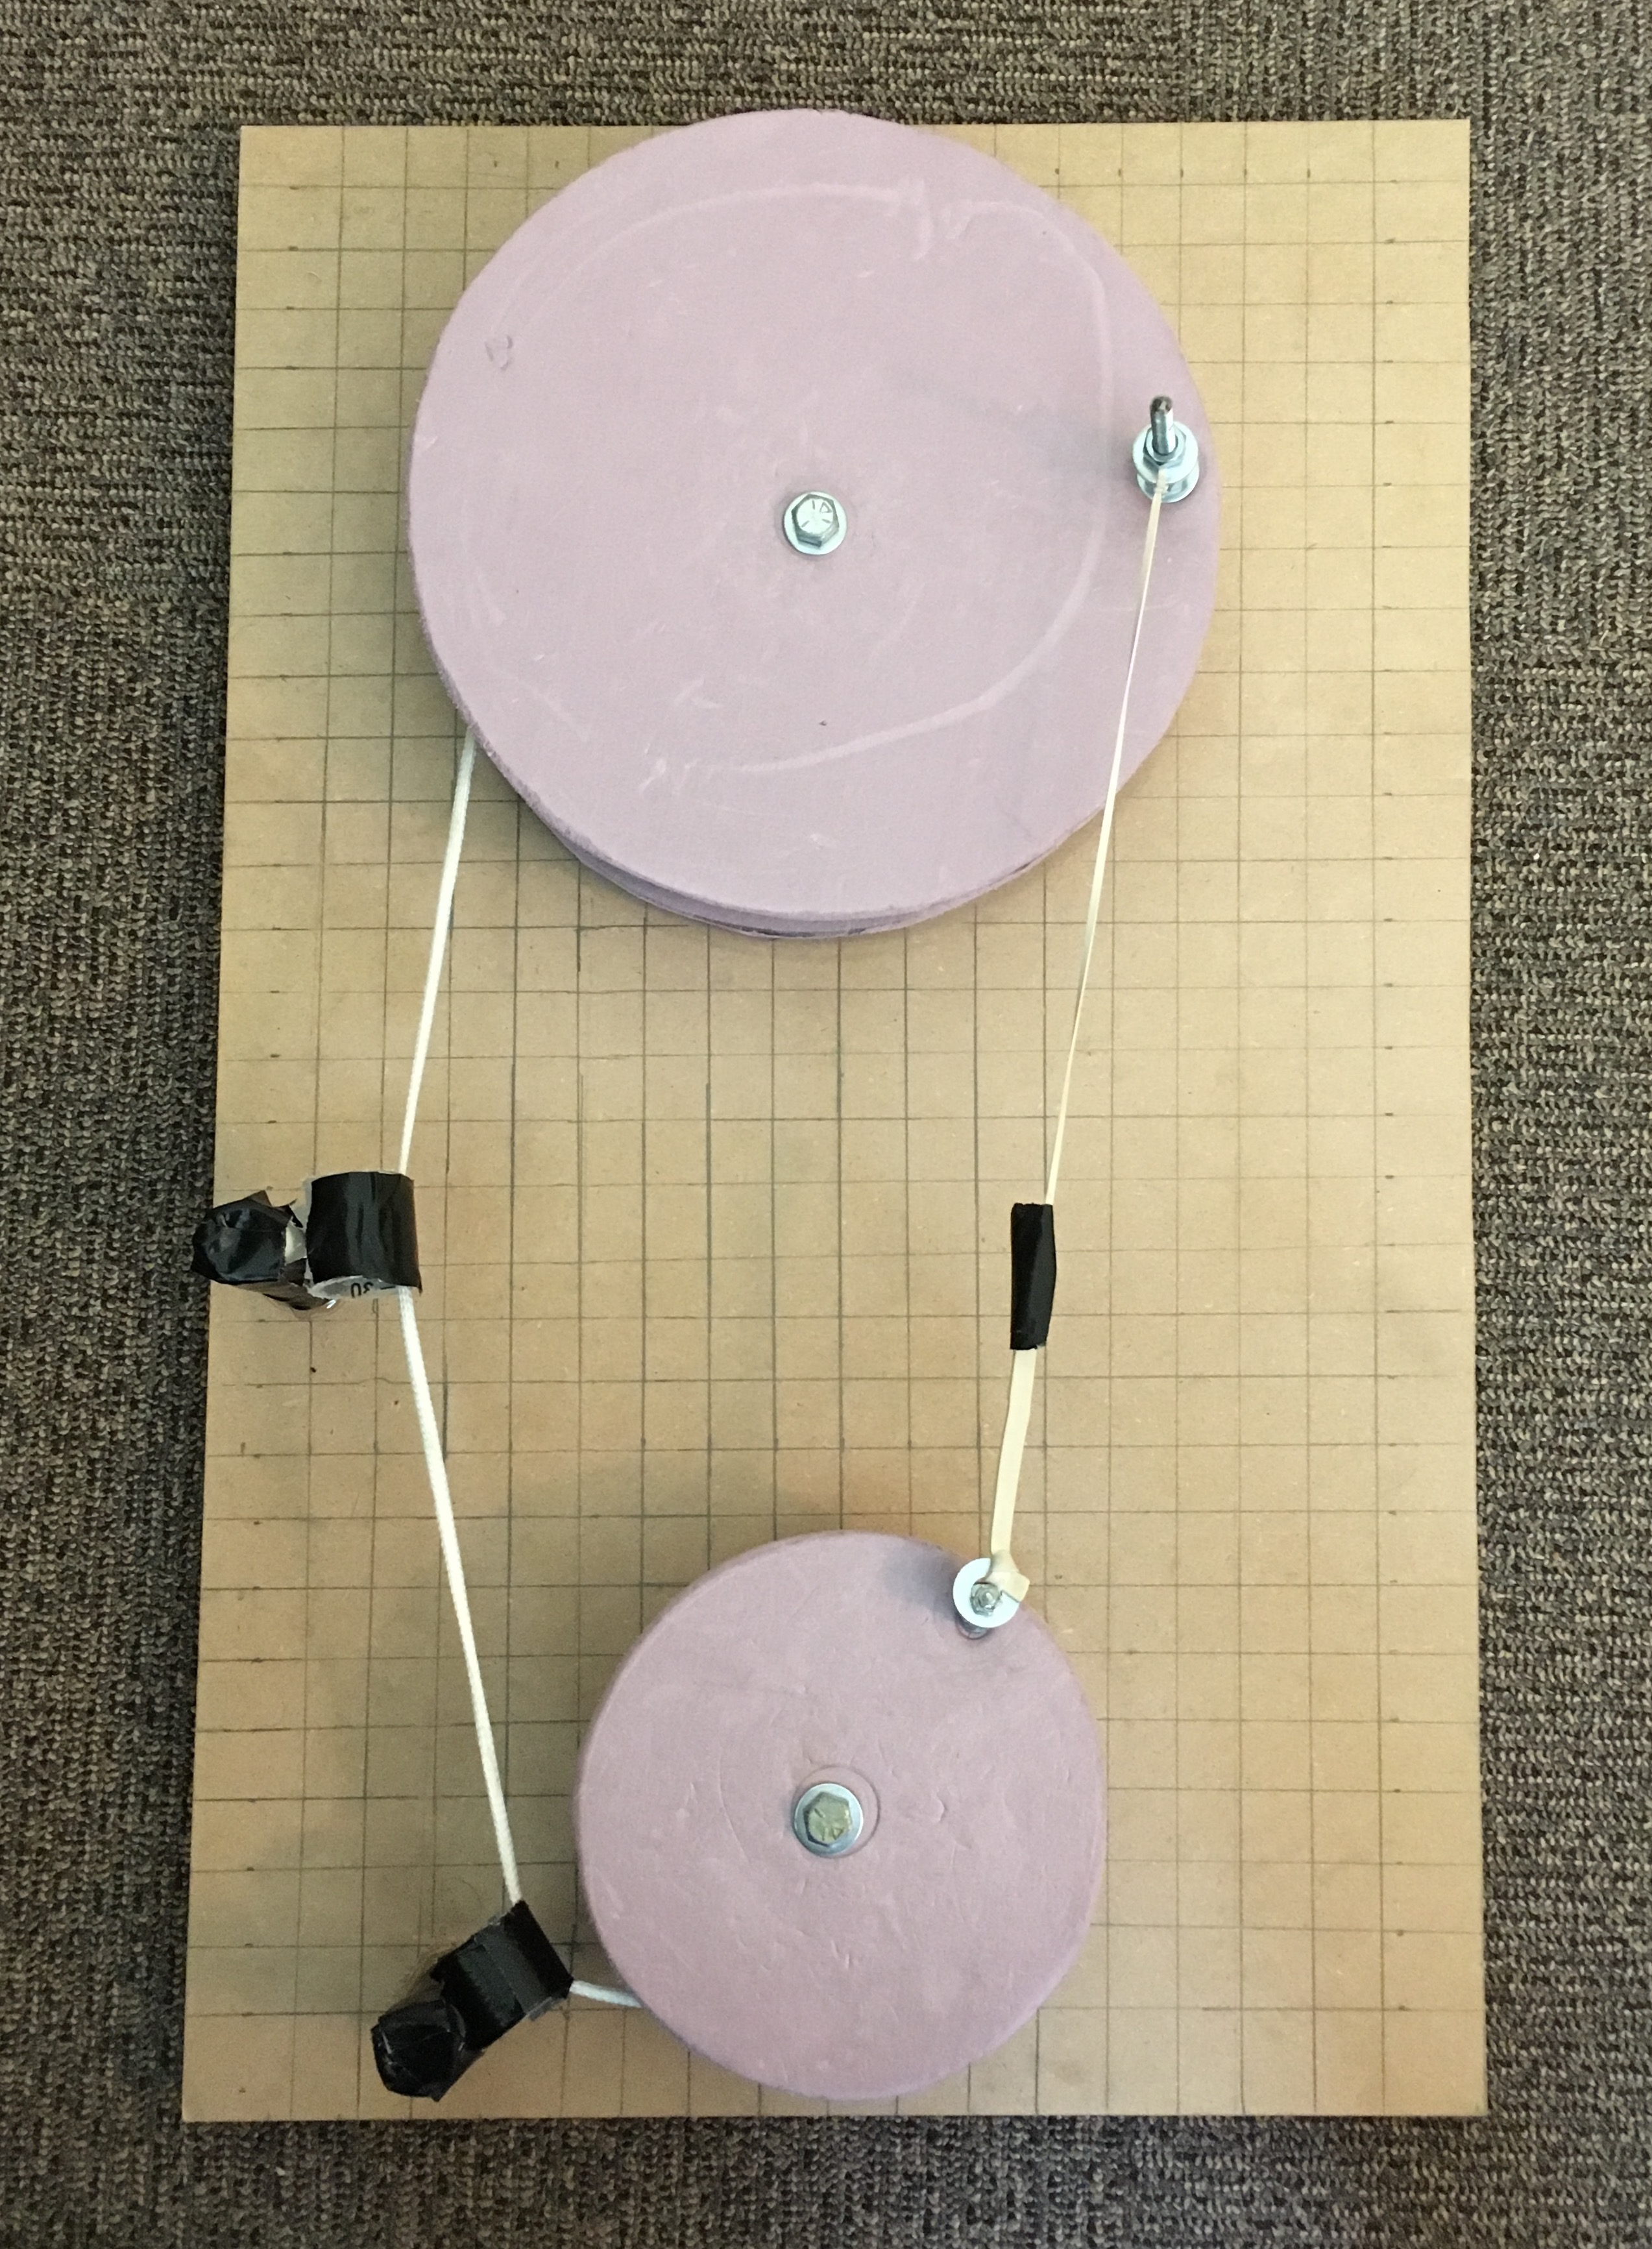
\includegraphics[width=0.35\textwidth]{prototype.jpg}
\end{figure}

%------------------------------------------------

% TODO @kevin: finish the prototype section
% Describe your prototype and any interesting things about how it was constructed, problems encountered, solutions you invented.
% Include a schematic diagram of the prototype
\section{Prototype}

\blindtext % Dummy text
%------------------------------------------------

% TODO @krishn: finish model
% Describe your BG, components, constitutive equations, and so on. Explain how you arrived at all the parameters you used. What  measurements did you take? How? Estimations and assumptions made? Theoretical calculations? Extraction of components and separate testing e.g. for springs?
\section{Model}

\begin{table}
\caption{Example table}
\centering
\begin{tabular}{llr}
\toprule
\multicolumn{2}{c}{Name} \\
\cmidrule(r){1-2}
First name & Last Name & Grade \\
\midrule
John & Doe & $7.5$ \\
Richard & Miles & $2$ \\
\bottomrule
\end{tabular}
\end{table}

\begin{equation}
\label{eq:emc}
e = mc^2
\end{equation}

\blindtext % Dummy text

%------------------------------------------------

% TODO @peter: finish this section
% What are your state variables and outputs of interest. Give matlab results (plots, not charts of numbers). Do NOT provide massive quantities of outputs. Be very selective and apply engineering acumen. One good output plot may be sufficient. Providing stacks of output plots is not necessary, in fact undesirable and would receive a lower grade. State variables themselves are often not interesting outputs.
\section{Simulation}

\blindtext % Dummy text

%------------------------------------------------

% TODO @peter: finish this section
% Compare simulation to data obtained from the system. Describe how well your simulation matches the actual behaviour as determined by an easily observable representative output variable (flashing lights, buzzer, counting rotations, and so on). Could the results be improved? Speculate on any significant descrepancies between test observations and simulation outputs. Explaining your validation process and demonstrating your understanding of the methods are much more important than getting wonderfully close agreement with the behaviour of your prototype.
\section{Discussion}

\blindtext % Dummy text


\end{document}
